\documentclass[a4paper,12pt]{article}
\usepackage[slovene]{babel}
\usepackage[utf8]{inputenc}
\usepackage{fullpage}
\usepackage{amsfonts} 
\usepackage{mathrsfs}
\usepackage[T1]{fontenc}
\usepackage{amsmath}
\usepackage[pdftex]{graphicx}
\usepackage[hidelinks]{hyperref}
\usepackage{bbm}
\usepackage{listings}
\usepackage{mathtools}
\usepackage{graphicx}
\usepackage{amssymb}




\begin{document}


\begin{center}
\huge \textbf{Občutljivost optimalne rešitve celoštevilskega linearnega programa}
\\[2cm]
\LARGE Poročilo
\\[2cm]
\end{center}


\section{Opis problema in način reševanja}


Za celoštevilski linearni program oblike
$$\max\left\{f^Tx; Ax \leq b, x \geq 0, x \in \mathbb{Z}^n \right\}$$
opazujeva občutljivost optimalne rešitve tega programa, glede na spremembe koeficietov $f$ in $b$. 
\\[0.5cm]
V projektu sva si na začetku izbrala začetni celoštevilski linearni program. Matriko $A$ fiksirala, vektorja $f$ in $b$ pa sva spreminjala. Pri tem sva opazovala kaj se zgodi z optimalnimi rešitvami problema, pri različnih koeficientih. Na enkrat sva spreminjala le en koeficient vektorja in pri tem vedno opazovala iteracije glede na začetni program. Za vsako spremembo koeficienta sva po več iteracijah opazovala optimalne rešitve. Te sva za vsak koeficinet prikazala v grafu, kjer sva originalno optimalno rešitev oziroma optimalno rešitev začetnega programa obarvala z drugo barvo. Naredila sva tudi graf, kjer so označene simulacije za celoten vektor, za vse koeficiente.
\\[0.5cm]
Za boljšo prestavo problema, sva naredila tudi primer dvorazsežne izbire vhodnih podatkov in narisala vizualizacijo v tri-dimenzionalnem grafu, kjer so zelo lepo vidne spremembe in učinki spreminjanja koeficientov.
\\[1cm]
Za programiranje sva si izbrala okolje Matlab. Morala sva narediti kodo za navaden celoštevilski linearni program. Za generacijo rezulatatov, sva se poslužila funkcije $intlinprog$, ki za argumente sprejeme osem vrednosti in spremenljivko z nastavitvami. Funkcija je namenjena mešanim linearnim programom, vendar se lahko uporablja tudi za celoštevilske linearne programe. Funkcija $intlinprog$ za reševanje linearnih programov uporablja metodo dual simplex. Glavna naloga pa je bila funkcija za spreminjanje koeficientov. To sva napisala na naslednji način:
\newpage
\lstset{language=Matlab} 
\begin{lstlisting}
Y=[];
h=1;
for i=1:4
     j=1;
     o=b(i);
     for n=1:s
          db=-10+20*rand();
          b(i)=b(i)+db;
          [x,fval]=intlinprog(f,intcon,A,b,Ae,be,[sp],[zg],options);
          B(i,j)=fval;
          B(i,j+1)=db;
          Y(:,h)=x;
          h=h+1;
	j=j+2;
	b(i)=o;
     end
end
\end{lstlisting}
Vhodne vrednosti, ki jih definiramo so:
\begin{itemize}
\item vektor $f$, ki predstavlja namensko funkcijo,
\item vektor $b$ in matriko $A$, ki skupaj definirata omejitve oblike $Ax \leq b$,
\item vektor $intcon$, ki določi spremenljivke v rešitvi $x$, ki morajo biti celoštevilske,
\item vektor $be$ in matriko $Ae$, ki definirata natančne omejitve oblike $(Ae)x=be$,
\item spremenljivka $s$, ki določa število iteracij,
\item vektorja $sm$ in $zm$, ki določita spodnje in zgornje meje rešitve $sm \leq x \leq zm$,
\item ter spremenljvka $options$, ki funksciji poda način reševanja problema in tolerance pri iteraciji, kjer sva midva rabila le nastavitev za obravnavanje celih števil.
\end{itemize}


Rešitve celoštevilskih linearnih programov sva shranjevala v matrikah $X$ oziroma $Y$ in $F$ oziroma $B$, ki sva jih pozneje razdelila na vektorje. V matriki $X$ oziroma $Y$ sva shranjevala rešitve celoštevilskega linearnega programa, ki sva jih v programu označila z $x$, v matrikah $F$ oziroma $B$, pa sva shranjevala optimalne vrednosti, ki sva jih označila v programu z $fval$, in spremembe koeficientov, ki sva jih označila z $df$ oziroma $db$.
\\[0.5cm]
V primeru analize občutljivost celoštevilskega linearnega programa v odvisnoti do omejitvene funkcije smo optimalne vrednosti in spremembe koeficientov shranili v matriko $B$. Vsaka vstica matrike prestavlja rezultate in motnje iteracij, pri katerih smo spreminjali korespondiran koeficient vektorja,  kjer so lihi členi optimalne vrednosti in sod členi spremembe koeficientov. Torej $B(3,:)$ predstavlja podatke po spreminjanju tretjega koeficienta vektorja $b$. V tem primeru smo otimalne reštitve shanili v matriko $Y$.


\section{Analiza občutljivosti celoštevilskega linearnega programa velikosti 4x4}

Za primer sva si izbrala celoštevilski linearni program, ki ima matriko $A$ velikosti 4x4 in vektorja $f$ in $b$ velikosti 4. Podatke sva izbrala čisto poljubno in naključno. Prikazala sva dva celoštevilska linearna programa, saj se je pri prvem programu zgodilo, da se optimalna rešitev ni spreminjala pod vplivom $f$-a(CLP-1). Pri drugem pa se optimalne rešitve na zanimiv način spreminjajo pod vplivom $f$-a(CLP-2).

\subsection{Analiza občutljivosti za CLP-1}

\begin{center}
$ A = \begin{bmatrix}
  1 & -2 & 3 & 4 \\
  9 & -3 & 4 & 5 \\
  1 & -3 & 5 & 7 \\
  2 & -4 & -5 & 1  
\end{bmatrix} $, $f=\begin{bmatrix} 10 \\10 \\10\\10 \end{bmatrix}$, $b=\begin{bmatrix} 12 \\12 \\12\\12 \end{bmatrix}.$
\\[0.5cm]
\end{center}

Naredila sva 40 iteracij. Določila sva interval, kjer se spremembe koeficientov naključno izbirajo in sicer $(-10,10)$, kar je bila najina izbira, saj lahko ta interval poljubno spreminjamo. 
\\[0.5cm]
Poglejmo si grafa, ki prikazijeta spremebe optimalne vrednosti ob spreminjaju
vektorja $b$:

\begin{figure}[h]
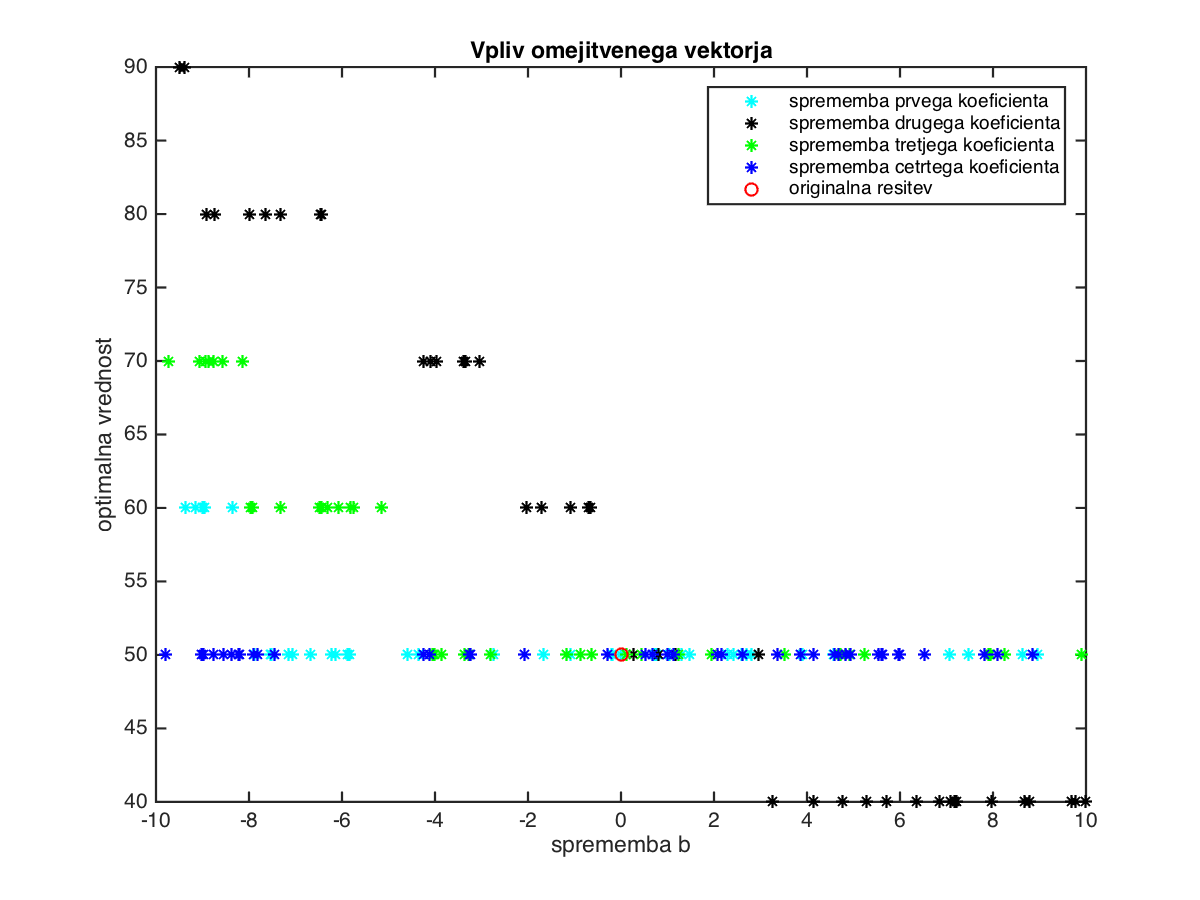
\includegraphics[width=14cm,height=10cm]{spremembe_b.png}
\end{figure}
\begin{figure}[h]
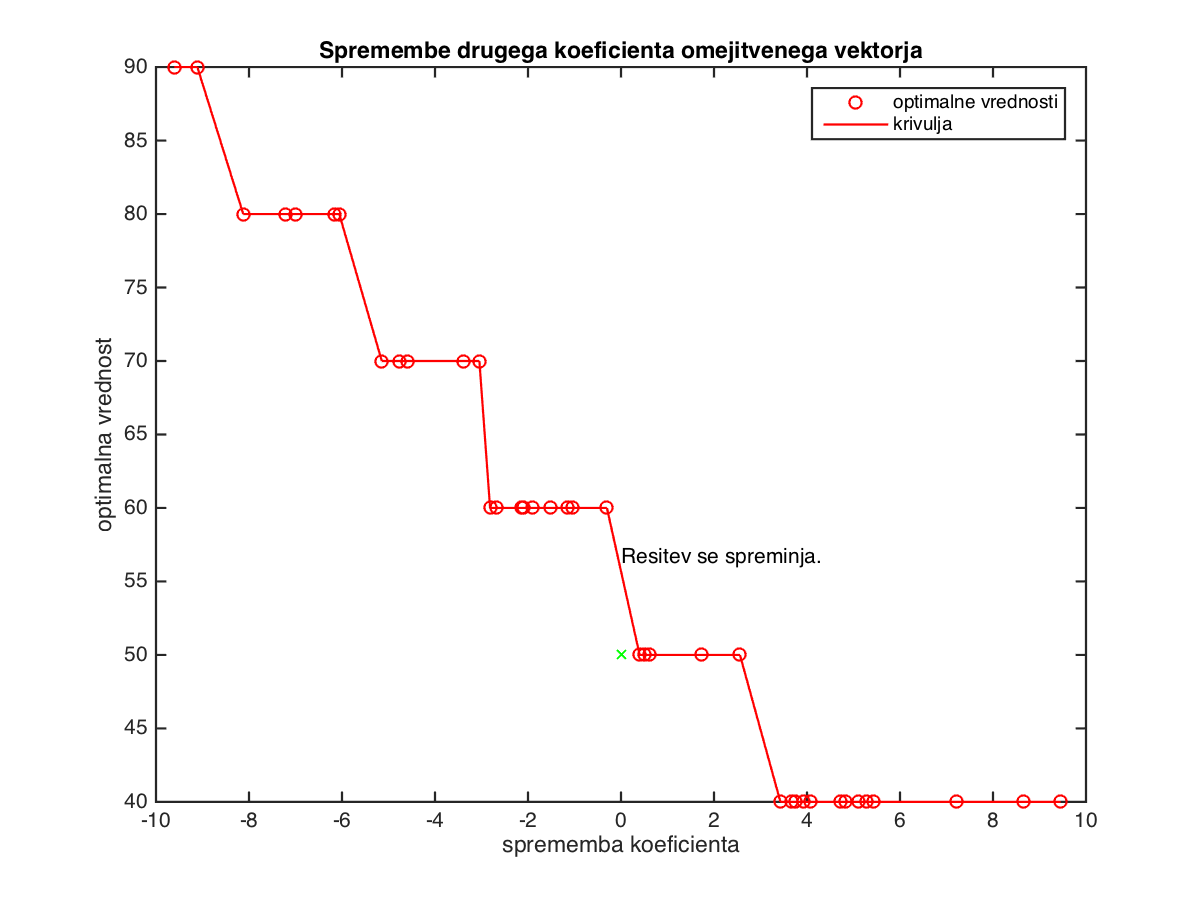
\includegraphics[width=14cm,height=10cm]{spremembe_b2.png}
\end{figure}

Iz prvega grafa je razvidno, da četrti koeficient na izbranem intervalu nima vpliva na optimalno vrednost in rešitev programa. S spremembo prvih treh koeficientov spreminjamo množico dopustnih rešitev, kar povzroča da se optimalna vrednost spreminja. Ker zahtevamo, da je optimalna rešitev celoštevilska, opazimo, da se optimalna vrednost spreminja za večkratnike koeficientov namenske funkcije. Za naš sprecifični program se je med analizo spreminjala le druga vrednost optimalne rešitve $x$. Zaradi tega se naša optimalna vrednost spreminja za večkratnike drugega koeficienta namenske funkcije. 
Ker imamo problem minimizacije, lahko opazimo, da se ob krčenju množice dopustnih rešitev optimalna vrednost viša. 


\newpage
\subsection{Analiza občutljivosti za CLP-2}

\begin{center}
$ A = \begin{bmatrix}
  2 & 6 & -3 & -3 \\
  2 & 4 & 1 & -1 \\
  -4 & -7 & -4 & -5 \\
   7 & -3 & -4 & -5  
\end{bmatrix} $, $f=\begin{bmatrix} -10 \\-10 \\-10\\ -10 \end{bmatrix}$, $b=\begin{bmatrix} 12 \\12 \\-12\\12 \end{bmatrix}.$
\\[0.5cm]
\end{center}

Za razliko od CLI-1 je zanimivo to, da je optimalna rešitev na intervalu $(-10,10)$ odvisna od $f$. Poglejmo si grafa, ki prikazijeta spremebe optimalne vrednosti ob spreminjaju vektorja $f$:

\begin{figure}[h!]
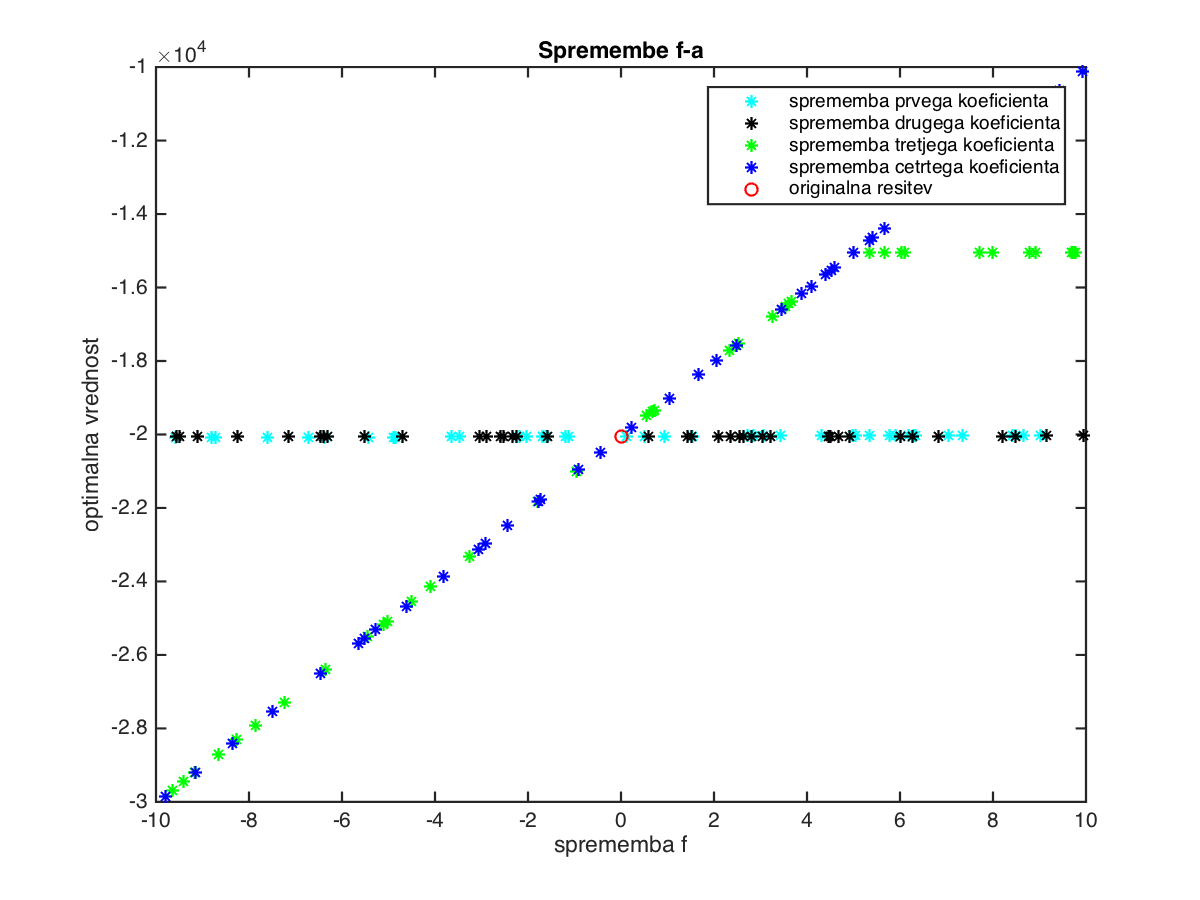
\includegraphics[width=11.2cm,height=8cm]{spremembe_f.png}
\centering
\end{figure}

Drugi in četrti koeficient nimata vpliva na optimalno rešitev na izbranem intervalu, prvi in tretji pa ga imata.
 
\clearpage

\begin{figure}[h!]
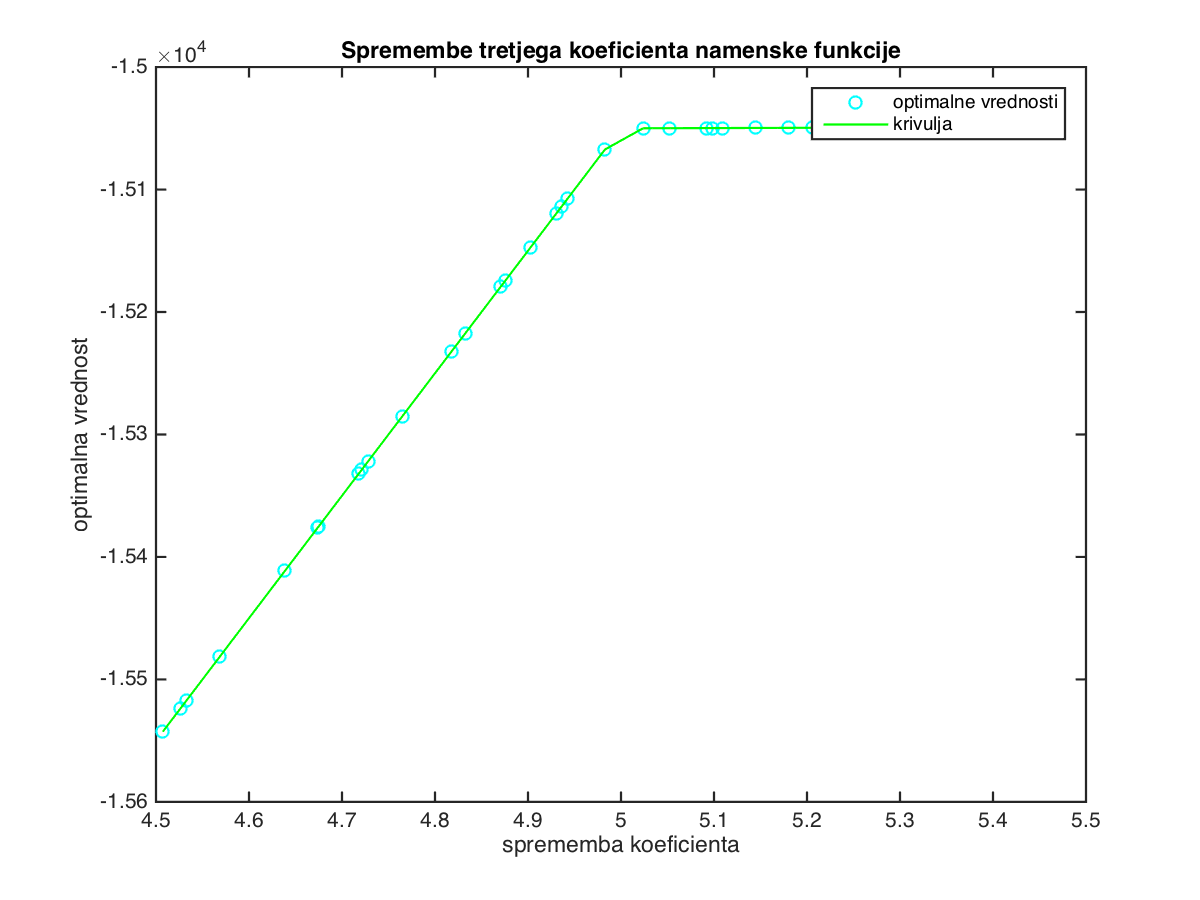
\includegraphics[width=11.2cm,height=8cm]{spremembe_f3.png}
\centering
\end{figure}

Iz grafa je razvidno, da se optimala rešitev spremeni. To lahko opazimo zaradi spremembe naklona. Koeficient $f$ se spreminja linearno, zato se optimalna vrednost spreminja linearno dokler je optimalna rešitev ista. 
Na intervalu ki smo si ga izbrali se optimalna rešitev spremeni, razlog za to lahko razložimo na spodnji sliki z naslovom $Vizualizacija za namensko funkcijo$. Premici predstavljata spreminjanje optimalne vrednosti pri dveh dopustnih rešitvah. Med njimi izberemo optimalno rešitev glede na to katera je manjša, saj imamo problem minimizacije. Zato bo optimalna rešitev zelena do $6$ in rdeča od $6$ dalje.

\begin{figure}[h!]
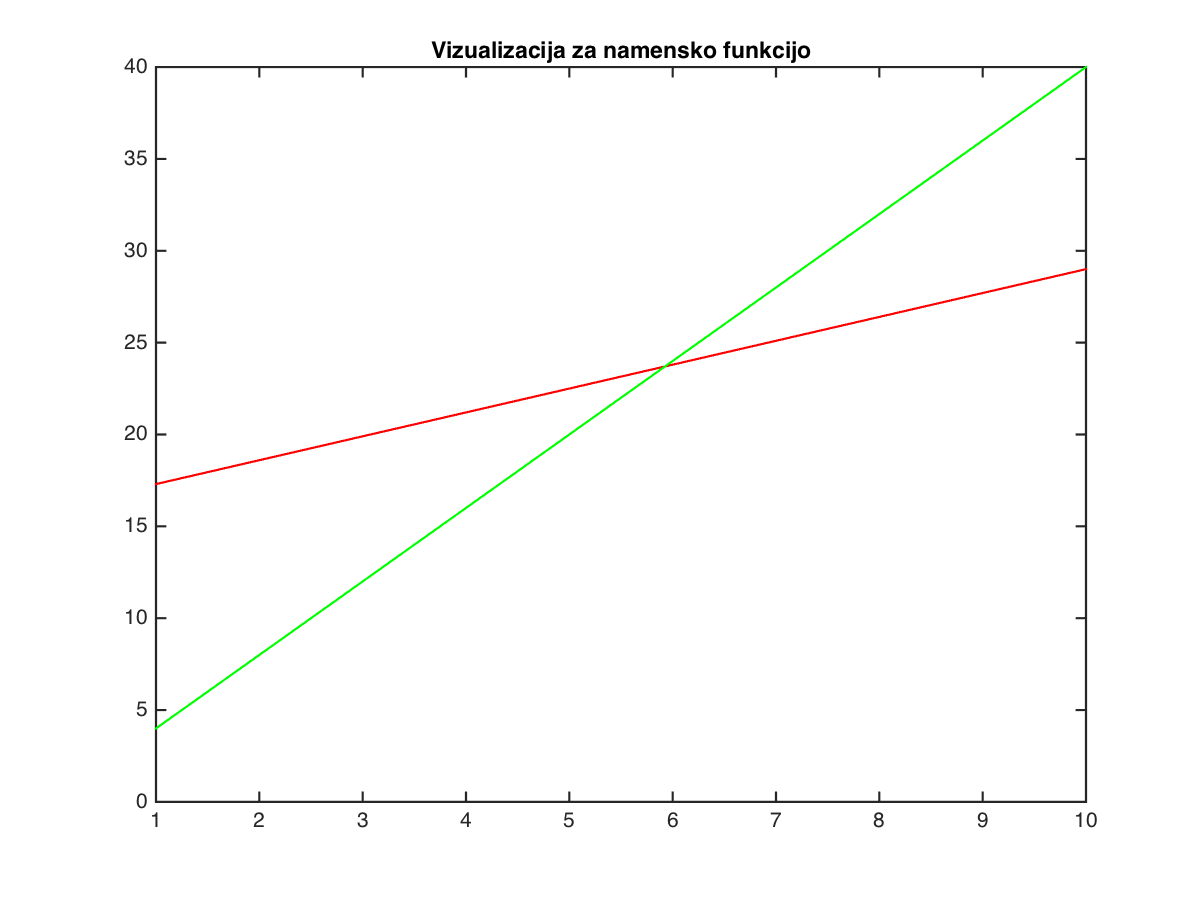
\includegraphics[width=12cm,height=8cm]{razlaga1.png}
\centering
\end{figure}


\clearpage

\section{Vizualizacija občutljivosti celoštevilskega linearnega programa}

Za boljšo predstavo učinkov namenskega in omejitvenega vektorja, sva analizirala celoštevilski linearni program velikosti 2x2:
\begin{center}
$ A = \begin{bmatrix}
  -3 & 1  \\
  2 & 1   
\end{bmatrix} $, $f=\begin{bmatrix} -4 \\ 6\end{bmatrix}$, $b=\begin{bmatrix} 3 \\ 10 \end{bmatrix}.$
\\[0.5cm]
\end{center}

Poglejmo si kakšen je grafični vpliv omejitvenega vektorja, pri čemer smo omejitveni vektor spremenili v $b=\begin{bmatrix} 3 \\ 8\end{bmatrix}$:

\begin{figure}[h!]
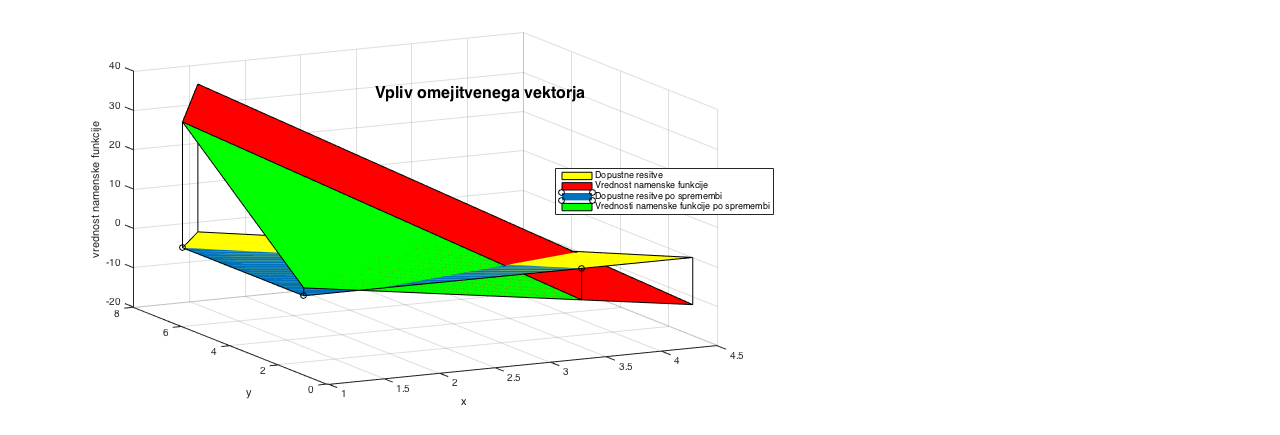
\includegraphics[width=15cm,height=10cm]{viz1.png}
\centering
\end{figure}
Optimana rešitev pred spremembo je $x=\begin{bmatrix} 4 \\ 1 \end{bmatrix}$, po spremembi pa je $x=\begin{bmatrix} 3 \\ 1\end{bmatrix}$. Optimalna vrednost $f^Tx$ je pred spremembo -10, po spremembi pa -6. Opazimo, da so vrednosti namenske funkcije ostale iste, vendar se je množica dopustnih rešitev skrčila. Zaradi tega je se je spremenila optimalna rešitev in optimalna vrednost.

\clearpage

Poglejmo si kakšen je grafični vpliv namenskega vektorja. Namenski vektor smo spremenili v $f=\begin{bmatrix} 1 \\ 6\end{bmatrix}$:

\begin{figure}[h!]
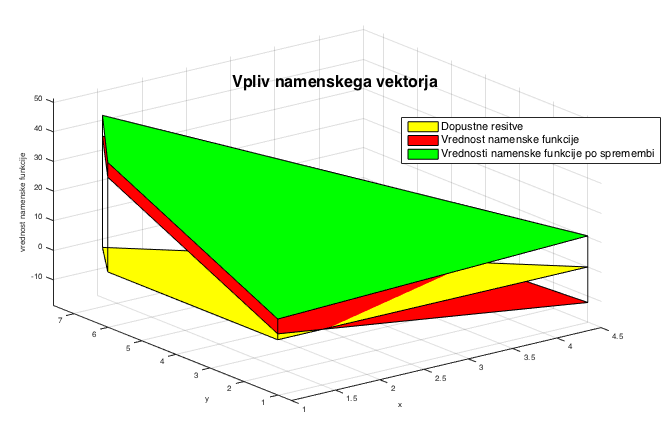
\includegraphics[width=15cm,height=10cm]{viz2.png}
\centering
\end{figure}

Optimana rešitev pred spremembo je $x=\begin{bmatrix} 4\\ 1\end{bmatrix}$, po spremembi pa je $x=\begin{bmatrix} 1 \\ 1 \end{bmatrix}$. Optimalna vrednost $f^Tx$ je pred spremembo -10, po spremembi pa 7.
Opazimo, da se vrednosti namenske funkcije spremenijo, medtem ko množica dopustnih rešitv ostane enaka.



\end{document}